
% LaTeX template for a Project Work (SNN-Unit)
% Version 5.0
% Copyright (C) 2015 Manuel Kohl, some rights reserved.
% Permission is hereby granted to freely copy, modify
% and/or redistribute this template under the terms and
% conditions of the Creative Commons Attribution License,
% either version 3.0 or, at your opinon, any later
% version of this License.
% For more detailed information, see
% http://creativecommons.org/licenses/by/3.0/

\documentclass[
    12pt,
    a4paper,
	chapterprefix=false,
	parskip=full,
	headings=normal,
	numbers=noenddot
]{scrreprt}

\usepackage[utf8]{inputenc}
\usepackage[english]{babel}
\usepackage[pdftex]{graphicx}
\usepackage{lmodern}
\usepackage[T1]{fontenc}

\usepackage{caption}
\usepackage{amsmath}
\usepackage[acronym]{glossaries}
\usepackage[numbers, square]{natbib}
\usepackage{microtype}

\usepackage{blindtext} % Remove this later

\usepackage[
	pdftitle={Project Work},
	pdfauthor={Max Mustermann},
	pdfcreator={\fmtname \space \fmtversion},
	pdfsubject={Subject of Project Work},
	pdfkeywords={}
]{hyperref}

\usepackage{listings}
\usepackage{color}
%Matlab color
\definecolor{mygreen}{RGB}{28,172,0} % color values Red, Green, Blue
\definecolor{mylilas}{RGB}{170,55,241}
%Csharp color
\definecolor{bluekeywords}{rgb}{0.13,0.13,1}
\definecolor{greencomments}{rgb}{0,0.5,0}
\definecolor{redstrings}{rgb}{0.9,0,0}
%Template color
\definecolor{darkblue}{rgb}{0.06275, 0.25882, 0.47843} % SNN-Unit color scheme

\hypersetup{
	colorlinks=true,
	frenchlinks=true,
	breaklinks=true,
	menucolor=black,
	linkcolor=darkblue,
	urlcolor=darkblue,
	citecolor=darkblue
}

\setkomafont{sectioning}{\normalfont\bfseries}
\setkomafont{descriptionlabel}{\normalfont\bfseries}

\def\registered{\textsuperscript{\textregistered}}
\def\trademark{\textsuperscript{\texttrademark}}

\makeglossaries

\newglossaryentry{abr}{
	name={ABR},
	description={The Auditory Brainstem Response is a type of time-locked stimulus-dependent evoked potential, which occurs in the acquired EEG signals within tens of milliseconds post stimulus}
}

\newglossaryentry{eeg}{
	name={EEG},
	description={The Electroencephalogram is a weak bioelectric signal originating from the electric sum activity of the apical dendrites of pyramidal neurons in the neocortex}
}

\begin{document}

\begin{flushright}
	
\includegraphics[width=4.5cm]{images/logo}
\end{flushright}

\begin{center}
	\vspace{\fill}
	\rule{\textwidth}{1pt}
	~\\
	\Large
	\textsc{VR Freifeld}\\
    \rule{\textwidth}{1pt}\\
    \vspace{\fill}
    \Large
	\textbf{Project Work}\\
	\vspace{\fill}
	\normalsize
	
	Saarland University of Applied Sciences\\
	Faculty of Engineering\\
    \vspace{\fill}
	\begin{tabular}{l l l}
		Submitted by & : & Dominik Limbach\\
		~ & ~ & ~\\
		Matriculation Number & : & 3662306\\
		~ & ~ & ~\\
		Course of Study & : & Biomedical Engineering\\
		~ & ~ & ~\\
		First Supervisor & : & Prof. Dr. Dr. Daniel J. Strauss\\
		~ & ~ & ~\\
		Second Supervisor & : & Dr. Lars Haab\\
	\end{tabular}
	~\\
	\vspace{\fill}
	Homburg, \today
\end{center}

\thispagestyle{empty}

\clearpage
\vspace*{\fill}
\small
\begin{center}

	Copyright \textcopyright \ \the\year \ Dominik Limbach, some rights reserved.
	
	\begin{minipage}{0.85\textwidth}
		Permission is hereby granted, free of charge, to anyone obtaining a copy of this material, to freely copy and/or redistribute unchanged copies of this material according to the conditions of the Creative Commons Attribution-NonCommercial-NoDerivatives License 4.0 International. Any form of commercial use of this material - excerpt use in particular - requires the prior written consent of the author.
	\end{minipage}
	
	
\includegraphics[width=4cm]{images/cc_by_nc_nd}
	
	\href{http://creativecommons.org/licenses/by-nc-nd/4.0/}{http://creativecommons.org/licenses/by-nc-nd/4.0/}

\end{center}
\normalsize
\thispagestyle{empty}
\clearpage

%\newpage


%\chapter*{Abstract}
%\addcontentsline{toc}{chapter}{Abstract}
%\setcounter{page}{1}

%
% Abstract

- a brief mentioning of the study and its attempt to treat acrophobia with a virtual environment\\
- theme of this thesis: the design of a VR fit to treat patients\\
- goal: evaluate the worth of a VR therapy by measuring changes in the subjects stress level(before/after)

%\newpage


%\chapter*{Zusammenfassung}
%\addcontentsline{toc}{chapter}{Zusammenfassung}

%
% Zusammenfassung

\blindtext


\newpage

\chapter*{Declaration}
\addcontentsline{toc}{chapter}{Declaration}

I hereby declare that I have authored this work independently, that I have not used other than the declared sources and resources, and that I have explicitly marked all material which has been quoted either literally or by content from the used sources. This work has neither been submitted to any audit institution nor been published in its current form.\\

\vspace{1cm}

Saarbrücken, \today\\

\vspace{1.5cm}

\underline{~ ~ ~ ~ ~ ~ ~ ~ ~ ~ ~ ~ ~ ~ ~ ~ ~ ~ ~ ~ ~ ~ ~}\\
\small
Dominik Limbach
\normalsize

\newpage

\renewcommand{\contentsname}{Contents}
\hypersetup{linkcolor=black}
\tableofcontents
\hypersetup{linkcolor=darkblue}

\newpage


\chapter{Introduction}


% Introduction

Der Präzedenzeffekt beschreibt die räumliche Zuordnung einer Schallquelle anhand der ersten Wellenfront die das Ohr erreicht. Dabei werden alle Folgeereignisse, die in einem gewissen Zeitbereich nach der ersten eintreffen ebenfalls der selben Richtung zugeordnet. Der Effekt tritt dann auf wenn zwei gleiche Schallereignisse mit einer Verzögerungszeit von 2-30 ms am Ohr ankommen und ist zudem abhängig vom Pegel der Folgeereignisse.\footnote{siehe \cite{ency},S.140ff}\footnote{siehe \cite{handbuch},S.103ff}\\
Solche Folgeereignisse sind zum großen Teil Reflexionen, die von den Wänden des Raumes zurückgeworfen werden. Reflexionen, die das Ohr nach einer zu langen Verzögerungszeit erreichen werden als Echo oder separates Schallereignis wahrgenommen. 
Aus diesem Grund werden akustische Messungen nicht selten im Freifeld durchgeführt.
Um diese Bedingungen zu realisieren bedarf es einer umfangreichen Schallisolation des Messraums. Dieser Umstand sorgt für zusätzliche Kosten und zu einer Beschränkung des
Versuchsaufbaus.
Die virtuelle Realität bietet eine kostengünstige Möglichkeit verschiedenste Messbedingungen zu simulieren und damit wissenschaftliche Experimente durchzuführen.
Wie sich nun eine Freifeld-Umgebung zur Durchführung von akustischen Messungen in der virtuellen Realität realisieren lässt ist Thema dieser Projektarbeit. 





\chapter{Problem Analysis and Goals}


% Problem Analysis and Goals

Bei akustischen Experimenten unter Freifeldbedingungen erfolgt die Präsentation der akustischen Signale in der Regel über Lautsprecher. Das Signal wird von der Versuchsperson entsprechend der Position des Lautsprechers im Raum wahrgenommen.\\
Im virtuellen Setup werden die akustischen Signale von einer virtuellen Quelle erzeugt, deren Position im virtuellen Raum der des realen Lautsprechers entspricht. Die Wiedergabe erfolgt jedoch in der Regel über einen Kopfhörer. Generell scheint ein Ton, der von einem Kopfhörer erzeugt wird, seinen Ursprung im Kopf zu haben. \\
Durch die Erzeugung eines virtuellen akustischen Raumes lässt sich die Anordnung der realen Schallquellen simulieren und somit eine räumliche Lokalisation der Schallquellen ermöglichen\footnote{siehe \cite{SLAS}}.
%Ziel ist die Simulation sämtlicher Eigenschaften der realen akustischen Umgebung mithilfe des
%virtuellen akustischen Raums.



\chapter{Materials and Methods}


% Materials and Methods
\section{Versuchsaufbau}
Die Grundlage des Versuchsaufbaus ist der virtuelle Raum in dem sich die Versuchsperson während der Durchführung aufhalten wird. Der Raum wurde mit Unity 5.6 von der Firma Unity Technologies erstellt.% google Link zu unity \\
Der Raum ist ein Würfel mit drei Metern Kantenlänge und einer Wandstärke von einem Zentimeter. Sämtliche Raumoberflächen besitzen den Standard Cube Mesh und einen Neutralen grauen Farbton. Die Umgebung wird mittels vier identischer Lichtquellen beleuchtet. Diese sind vom Typ Spotlight und sind mit einem Winkel von plus neunzig Grad zu der Decke auf den Boden gerichtet. Um eine ausgeglichene Beleuchtung, ohne Überstrahlung, an den Kanten des Raumes zu gewährleisten befinden sich die Lichtquellen in einem Abstand von zwei Metern oberhalb der Raumdecke und ihre Intensität wurde auf achtzig Prozent eingestellt. Für den Benutzer werden die Lichtquellen durch vier Deckenlampen dargestellt.\\
Die Gestaltung wurde bewusst schlicht gehalten, da die Realitätsnähe nicht im Fokus des Experimentes lag.\\
Darüber hinaus enthält der virtuelle Raum das Setup für den Freifeldversuch.
Es besteht aus vier virtuellen Lautsprechern, einem virtuellen Mikrofon, einem visuellen Hinweis und einer zentralen Markierung für den Probanden auf dem Boden.\\
% AudioSources
Die Audioquellen, wurden in Form spezieller Game Objects innerhalb der Unity Umgebung implementiert. Diese heißen Audio  Source und sind in der Lage einen beliebigen Audio Clip wiederzugeben\footnote{siehe \cite{UnityManualAudioSource}}.% Unity User Manual AudioSource
Um die Position jeder Audio Source im Raum erkennen zu können wurden sie jeweils mit dem 3D-Modell eines Lautsprechers verknüpft. Jeder dieser virtuellen Lautsprecher  wurde auf einem kleinen Podest positioniert. Die vier Audioquellen befinden sich auf einer Kreisbahn um die Probanden Markierung mit einem Radius von zwei Metern.\\
Die Positionen der vier Quellen sind wie folgt:
\begin{itemize}
\item Links Lateral: $-90^{\circ}$
\item Links Frontal: $-30^{\circ}$
\item Rechts Frontal: $+30^{\circ}$
\item Rechts Lateral: $+90^{\circ}$
\end{itemize}
Der Abstand der virtuellen Lautsprecher zum Boden beträgt 1,20 Meter. \\
Die Audioquellen sind mithilfe des audio spatializer plugin, welches direkt in Unity implementiert ist, in der Lage die Wiedergabe des Audio Clip so zu beeinflussen, dass dieser seiner Position im virtuellen Raum entsprechend wahrgenommen werden kann. Die Aktivierung dieser Funktion erfolgt über den Unity Audio Manager\footnote{siehe \cite{Spatial}}.\\
Dieser muss wie folgt konfiguriert werden:
\begin{itemize}
\item Default Speaker Mode: Stereo
\item System Sample Rate: 48000 Hz
\item Spatializer Plugin: MS HRTF Spatializer
\end{itemize}
Die restlichen Einstellmöglichkeiten verbleiben auf den Standardwerten.\\
Darüber hinaus muss jede der erstellten Audioquellen entsprechend konfiguriert werden.
\begin{itemize}
\item Spatialize: On
\item Volume: 1
\item Stereo Pan: 0
\item Spatial Blend: 1
\item Spread: 0
\end{itemize}
Unity bietet dem Nutzer an dieser Stelle mit der Volume Rolloff Einstellung die Möglichkeit jede der oben genannten Parameter innerhalb des Einflussbereichs der Audioquelle, abhängig von der Entfernung des Hörers zur Quelle, zu beeinflussen.\\
Im Rahmen dieses Aufbaus wurde ein Custom Rolloff gewählt, welcher zu einer Dämpfung des Signals innerhalb eines Radius von acht Metern um die Quelle führt. Dies kann dem Probanden während des Versuch zusätzliche Informationen über seine Entfernung zu der jeweiligen Quelle geben. Die restlichen, der oben genannten Parameter, bleiben innerhalb des gesamten Einflussbereichs der Quelle unverändert.\\
% AudioListener
Der von den Audioquellen abgespielte Audio Clip wird von einem virtuellen Mikrophon aufgezeichnet. Dieses Mikrofon ist in Form des Audio Listeners in der Unity Engine implementiert und ist nicht konfigurierbar. Er wurde als eine Komponente des Kopfkamera, der sogenannten camera(ears), angelegt. Somit wird jede Ausgabe der Audioquellen aus der Sicht des Trägers der VR-Brille wahrgenommen.\\
Der visuelle Hinweis wurde in Form eines grünen Pfeils implementiert. Dieser befindet sich an der Wand des virtuellen Raumes, welche sich hinter den Audioquellen befindet. Seine Position entspricht $0^{\circ}$ auf der Kreisbahn und sein Abstand zum Boden beträgt 1,20 Meter.

\newpage
Abschließend wurde das HTC Vive kalibriert, der Untersuchungsraum vermessen und ein Stuhl auf der Markierung platziert.
% Methoden
\section{Versuchsablauf}
\subsection{Vorbereitung Proband/in}
Nachdem der/die Proband/in über den Ablauf informiert wurde wird er/sie angewiesen sich zur Markierung zu begeben und Platz zu nehmen. Anschließend wird ihm/ihr die VR-Brille und Kopfhörer aufgesetzt und entsprechen fixiert.

\subsection{Ablauf}
Zu Beginn des Experiments werden die Untersuchungsparameter durch den Versuchsleiter eingegeben. Über ein Matlab Programm, welches auch die Eingabe verwaltet, wird das Wiedergabeprotokoll erstellt, die Untersuchungsdaten gespeichert und an Unity übergeben.
Das Wiedergabeprotokoll wird entsprechend der eingegebenen Parameter automatisch erstellt.
Für jedes wiederzugebende Signal wird eine zufällige Quelle zur Wiedergabe bestimmt.\\
Sobald das Protokoll erstellt und and Unity gesendet worden ist kann das Experiment gestartet werden.\\
Während des Experiments wird der Versuchsperson eine Folge von akustischen Signalen präsentiert. Der/Die Proband/in wird angewiesen nach jeder Signalwiedergabe die Richtung aus der das Signal wahrgenommen wurde anzugeben. Nachdem das Programm gestartet wurde
wird der ausgewählte Audio Clip in einem fünf Sekunden Intervall von jeweils einer der vier Audioquellen wiedergegeben. Zu jeder Wiedergabe wird der Versuchsperson ein visueller Hinweis in Form einer Richtungsangabe durch einen grünen Pfeil in ihrem Sichtfeld dargeboten. Das Programm ist beendet, wenn die gewünschte Signalanzahl erreicht wurde.

\newpage
\section{Code}
\subsection{Matlab}
\lstset{language=Matlab,%
    %basicstyle=\color{red},
    breaklines=true,%
    morekeywords={matlab2tikz},
    keywordstyle=\color{blue},%
    morekeywords=[2]{1}, keywordstyle=[2]{\color{black}},
    identifierstyle=\color{black},%
    stringstyle=\color{mylilas},
    commentstyle=\color{mygreen},%
    showstringspaces=false,%without this there will be a symbol in the places where there is a space
    numbers=left,%
    numberstyle={\tiny \color{black}},% size of the numbers
    numbersep=9pt, % this defines how far the numbers are from the text
    emph=[1]{for,end,break},emphstyle=[1]\color{red}, %some words to emphasise
    %emph=[2]{word1,word2}, emphstyle=[2]{style},    
}

\lstinputlisting{freifeld.m}

\newpage
\subsection{Unity}

\lstset{language=[Sharp]C,
showspaces=false,
showtabs=false,
breaklines=true,
showstringspaces=false,
breakatwhitespace=true,
escapeinside={(*@}{@*)},
commentstyle=\color{greencomments},
keywordstyle=\color{bluekeywords}\bfseries,
stringstyle=\color{redstrings},
basicstyle=\ttfamily
}

\lstinputlisting{UnityServerLatex.cs}

\newpage

\lstinputlisting{ArrayControlLatex.cs}




%\chapter{Results}

%
% Results
\section{Electrodermal Activity}

We have plotted the average SCL of all subjects during the baseline and exposure measurement in the form of boxplots, as can be seen in figure \ref{SCLbpImg}. Additionally we included the overall average differences in SCL between the two measurements.
 
\begin{figure}[h]
\centering
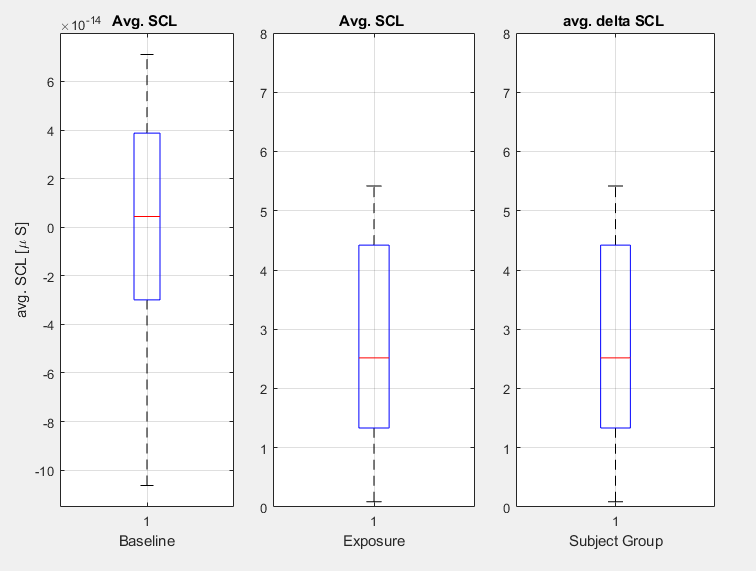
\includegraphics[width=1\textwidth]{images/avgSCL.png}
\caption{Boxplot comparison of the average SCL in subject's baseline (left) and exposure measurement (middle) as well as the average difference in the SCL of the two measurements (right).}
\label{SCLbpImg}
\end{figure}

\newpage
In figure \ref{EDAbpImg} the peak interval distributions of each subject were illustrated in the form of a boxplot for both the baseline and the exposure measurement. The median RR interval is indicated by a red, horizontal line inside the box. The lower and the upper quartile are displayed by the lower and upper edge of the box, respectively. Minimum and maximum value of the peak interval sample are indicated by the endpoints of the, so called, whiskers (outliers are marked as red +).

\begin{figure}[h]
\centering
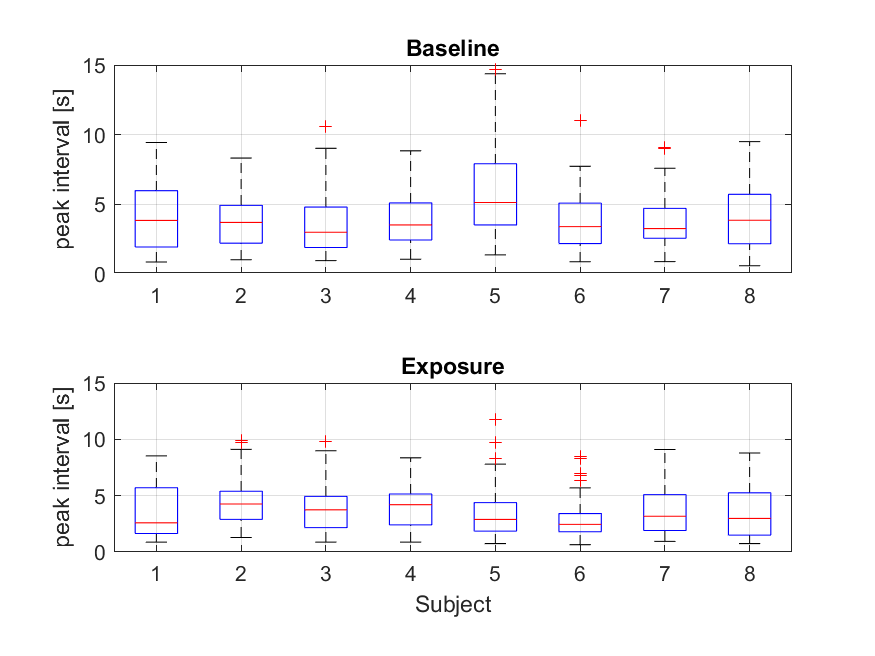
\includegraphics[width=1\textwidth]{images/EDApid.png}
\caption{Boxplot comparison of the peak interval distribution of subject's baseline and exposure EDA measurement.}
\label{EDAbpImg}
\end{figure}

\newpage
An example of an alternative way to illustrate the peak interval distribution is shown in figure \ref{SCLbpImg}. We have created histograms for each subject indicating the frequency of the measured peak intervals. 

\begin{figure}[h]
\centering
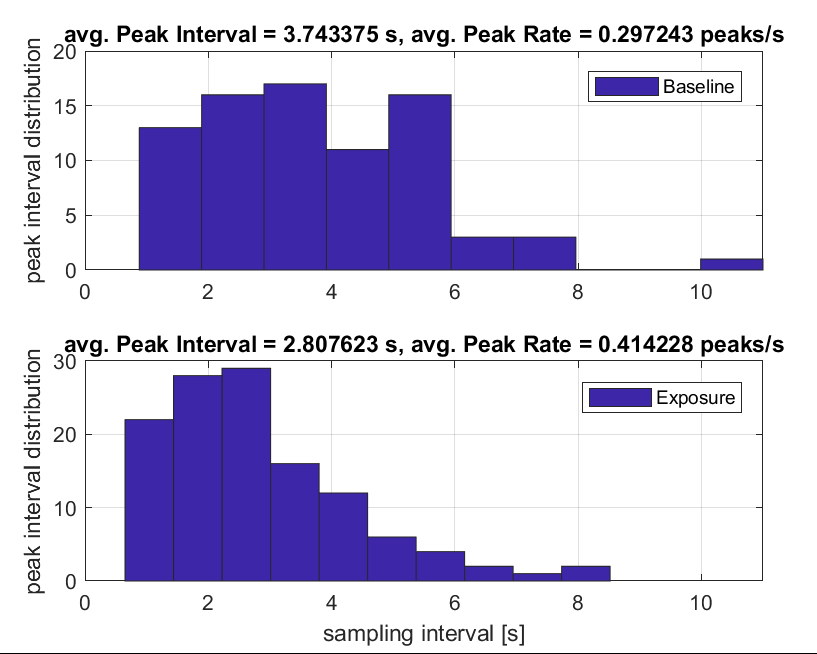
\includegraphics[width=1\textwidth]{images/EDAhisto.png}
\caption{Histogram, illustrating the peak interval distribution of a subject's baseline and exposure EDA measurement.}
\label{EDAhistoImg}
\end{figure}

\newpage
\section{Electrocardiogram}
According to the illustration of EDA, the RR intervals of all subjects are presented in similar fashion in figure \ref{ECGbpImg}. As well as the individual RR distribution in figure \ref{ECGhistoImg}.

\begin{figure}[h]
\centering
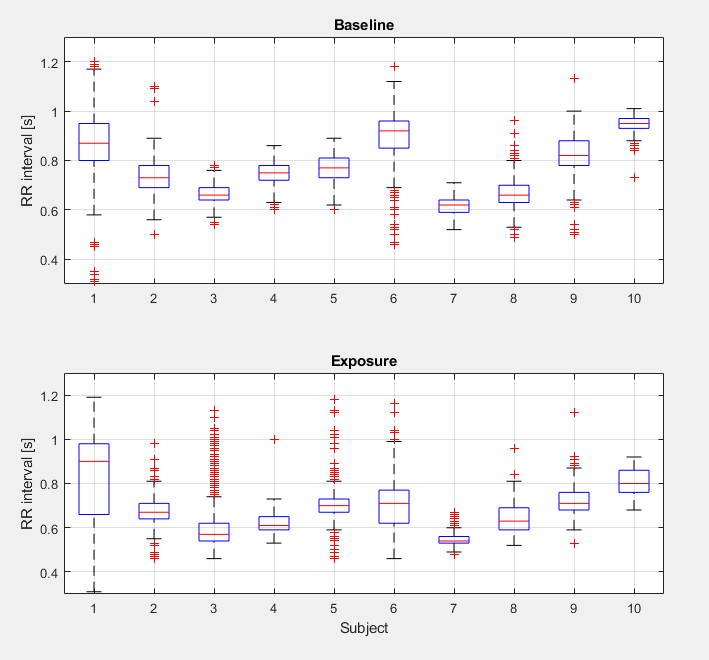
\includegraphics[width=1\textwidth]{images/ECGRRp.png}
\caption{Boxplot comparison of the RR interval distribution of subject's baseline and exposure ECG measurement.}
\label{ECGbpImg}
\end{figure}

\begin{figure}[h]
\centering
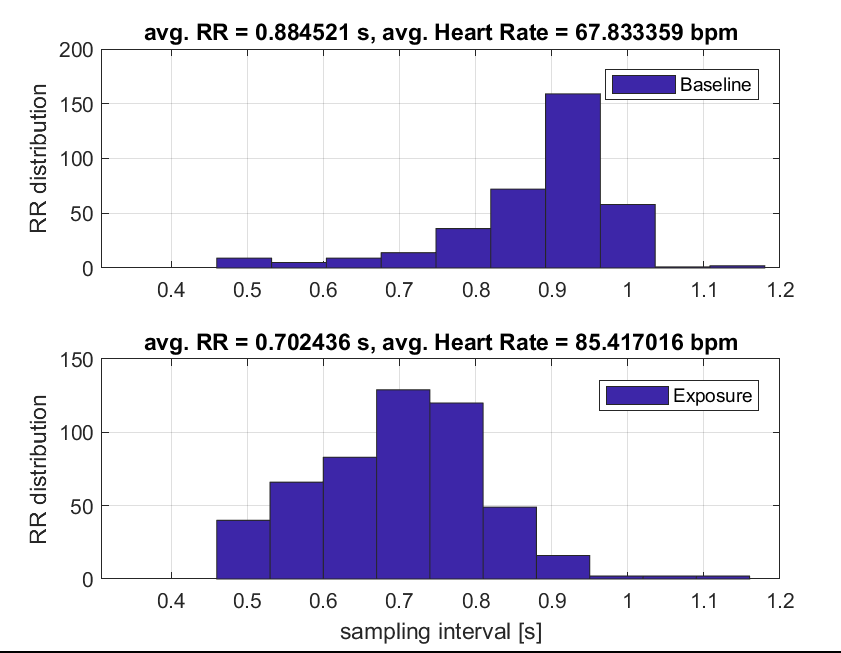
\includegraphics[width=1\textwidth]{images/ECGhisto.png}
\caption{Histogram, illustrating the RR interval distribution of a subject's baseline and exposure ECG measurement.}
\label{ECGhistoImg}
\end{figure}

\newpage
%\begin{landscape}
\section{Statistical Results}

\subsection{Shapiro-Wilk Test}
Apart from one exception the null hypothesis has been confirmed for all samples. The null hypothesis has been rejected for the baseline peak interval sample. All tests were conducted with a significance level of 5\%.

The parameter as well as the results of the Shapiro-Wilk test are shown in table \ref{shapirowilk}, including sample size (n), confidence level ($\alpha$), test statistic (W) as well as its critical value ($W_{critical}$), mean value ($\bar{x}$) for each sample (x), weight coefficients ($a_{i}$) and eventually the test result (H). The null hypothesis was confirmed for all W greater than $W_{critical}$. The confirmation of the null hypothesis is indicated through H=0, whereas its rejection is indicated by H=1.

\begin{table}[h]
\centering
\caption{Results: Shapiro Wilk test}
\begin{tabular}{|c|c|c|c|c|c|c|c|}
\hline
sample x & n & $\alpha$ & W & $W_{critical}$ & $\bar{x}$ & $a_{i}$ & H\\
\hline
EDA BL & 8 & 0.05 &  0.6621 & 0.818 & 4.1107 & 0.6052 0.3164 0.1743 0.0561 & 1\\
\hline
EDA EP & 8 & 0.05 &  0.8318 & 0.818 & 4.0032 & 0.6052 0.3164 0.1743 0.0561 & 0\\
\hline
SCL BL & 8 & 0.05 &  0.8476 & 0.818 & -1.0882e-15 & 0.6052 0.3164 0.1743 0.0561 & 0\\
\hline
SCL EP & 8 & 0.05 &  0.9511 & 0.818 & 3.3930 & 0.6052 0.3164 0.1743 0.0561 & 0\\
\hline
ECG BL & 10 & 0.05 & 0.9596 & 0.842 & 0.7720 & 0.5739 0.3291 0.2141 0.1224 0.0399 & 0\\
\hline
ECG EP & 10 & 0.05 & 0.9650 & 0.842 & 0.6834 & 0.5739 0.3291 0.2141 0.1224 0.0399 & 0\\ 
\hline	
\end{tabular}
\label{shapirowilk}
\end{table}

%
%\thispagestyle{empty}
%\clearpage
%\end{landscape}
%
%\newpage

\subsection{Two-Sample T-test for paired Samples}
The null hypothesis was confirmed for the EDA peak interval samples and rejected for SCL mean samples as well as ECG RR interval samples. In table \ref{ttest} all parameters of the t-test and its results are listed, including sample size (n), confidence level ($\alpha$), degrees of freedom (df), rejection value ($V_{out}$) as well as the mean difference (d) and eventually the test results t-value and H. The null hypothesis was rejected for t-values greater than ($V_{out}$). The confirmation of the null hypothesis is indicated through H=0, whereas its rejection is indicated by H=1.

\begin{table}[h]
\centering
\caption{Results: two-sample t-test}
\begin{tabular}{|c|c|c|c|c|c|c|c|}
\hline
sample x & n & $\alpha$ & df & $V_{out}$ & d & t & H\\
\hline
EDA  & 8 & 0.05 &  7 & 1.895 & 0.1074 & 0.2175 & 0\\
\hline
SCL  & 8 & 0.05 &  7 & 1.895 & 3.3930 & 2.9112 & 1\\
\hline
ECG  & 10 & 0.05 & 9 & 1.833 & 0.0886 & 5.8845 & 1\\
\hline	
\end{tabular}
\label{ttest}
\end{table}

\subsection{Effect Size}
The effect size d, or Cohen's d, of the two-sample t-test as well as the correlation coefficient r are shown in table \ref{effecttest}. In addition all associated test parameter, including the samples, sample size (n), sample means and pool variance ($\sigma$) were listed.

\begin{table}[h]
\centering
\caption{Results: effect size test}
\begin{tabular}{|c|c|c|c|c|c|c|c|}
\hline
sample 1& sample 2 & n & mean 1 & mean 2 & $\sigma$ & d & r\\
\hline
EDA EP & EDA BL & 8 & 4.0032 & 4.1107  & 0.9150  & 0.1174 & 0.0073 \\
\hline
SCL BL & SCL EP & 8 & -1.0882e-15 &  3.3930 & 2.3310 & 1.4556 & 0.0906 \\
\hline
ECG EP & ECG BL & 10 & 0.6834 & 0.7720 & 0.0983 & 0.9010 & 0.0450 \\
\hline	
\end{tabular}
\label{effecttest}
\end{table}



\chapter{Discussion}


% Discussion
\section{Data Acquisition Quality}
We have obtained 22 sets of data, 11 for each EDA and ECG, of the 11 subjects that were measured in our experiment. Three EDA measures were rejected due to exceeding the imaging range of the BITalino device of 0-25 $\mu S$. The 3 data sets correlate with the subjects that stated increased palmar sweating. We also had to eliminate 1 ECG measure due to immense motion artifacts, which although expected to some degree were to frequent and likely caused by contact of the electrode cables to the subject's legs. To ensure higher efficiency in future measures involving the BITalino (r)evolution it is recommended to increase attention on cable management and reconsider palmar electrode placement for ECG measurements, which are particularly prone to motion artifacts.

\section{Sympathetic Activation}
Earlier, we have highlighted the connection between sympathetic activation and psychophysiological measures, particularly heart rate variation and tonic components of the EDA. It is suggested that an activation of the sympathetic nervous system is caused by the presence of a stimulus and reflected by an increase of these measures. We have chosen to indicate the heart rate in the form of RR intervals. Thus, an increase in heart rate, caused by a stimulus, is equal to a decrease in RR distance. As shown in figure \ref{ECGbpImg} the exposure has caused an overall decrease in RR distance in all subjects. This effect can also be found in figure \ref{ECGhistoImg}, where the RR distribution of, both, the baseline and the exposure measurement of a single subject (see \ref{ECGbpImg}) was mapped in the form of a histogram, to illustrate the drift towards lower RR distances during the exposure. In addition the average heart rate, which is shown on top of each histogram (see \ref{ECGhistoImg}) increase significantly.
The same effect could be observed in EDA measures (see \ref{EDAbpImg}, \ref{EDAhistoImg}), as the average peak interval time decrease and the peak rate of NS-SCRs increased. When comparing the average differences in SCL between the two phases, we found an observable increase during the exposure (see \ref{SCLbpImg}). Therefore, we are able to conclude our virtual environment to be sufficiently stimulating and the offered stimulus are considered effective. 

\section{Statistic Evaluation and Feature Quality}

To evaluate the possible use of the extracted features we have conducted a two-sample t-test for paired samples. As mentioned earlier, this test was designed around the null hypothesis $H0: \mu_{X}-\mu_{Y} = \omega_{0}$, where we assume $\omega_{0}=0$ and therefore impute that there will be no difference between two measures of the same subject. This hypothesis has been disproved for SCL and RR interval measurements. Therefore we have shown that there is a significant increase in these features during the exposure. In addition, we gathered information on effect size of the t-test, using the Cohen's d, and therefore the practical significance of a significant difference in the mean values. With d values of 1.4556 for SCL and 0.9010 for RR distance we distinctly exceed the criteria of a strong effect (d > 0.8). This means that an increase in both signal features is likely to be observed. Thus, we acknowledge the quality of the average change in SCL and the average RR interval for the real-time assessment of an individual's mental state, particularly the sympathetic fear reaction.\\
There are however some conditions to the application of the two-sample t-test. The most important one being that the samples are derived from populations with normal distribution. Thus, we performed a test on normality with the null hypothesis H0, which states that population of the tested sample possesses a normal distribution. We have confirmed H0 for all both ECG and SCL and therefore assume the results of the t-test to be justified. On the other hand the t-test for EDA peak intervals yielded positive results (this means H0 was confirmed). Therefore no significant difference between baseline and exposure was found. How strongly this is effected by the associated baseline sample failing the Shapiro-Wilk test and the time difference of the two measurements could not be determined. However, the test results suggest the elimination of average peak interval as a quality feature in the detection of sympathetic activation during the exposure.  


\chapter{Conclusions and Future Work}


% Conclusions and Future Work

%zusammenfassend
%
%vr < freifeld
%vr jedoch günstig und mobil
Abschließend lässt sich sagen, dass mit einem VR-Setup zwar zufriedenstellende Ergebnisse zu erzielen sind. In der Realität ist es jedoch sehr schwer die Qualität eines konventionellen Aufbaus zu erreichen. Bei der Entscheidung für ein VR-Setup spielen vor allem niedrige Kosten, Ortsungebundenheit und Vielseitigkeit eine tragende Rolle. Bestehen hohe Qualitätsansprüche bezüglich der räumlichen Lokalisation ist nach wie vor Freifeld Setup mit entsprechender Hardware zu bevorzugen.

%\appendix

%
% Appendix

\chapter{Tables and Measurement Results}



\newpage


%\addcontentsline{toc}{chapter}{List of Figures}
%\hypersetup{linkcolor=black}
%\listoffigures
%\hypersetup{linkcolor=darkblue}

%\newpage
%
%\addcontentsline{toc}{chapter}{List of Tables}
%\hypersetup{linkcolor=black}
%\listoftables
%\hypersetup{linkcolor=darkblue}
%
%\addcontentsline{toc}{chapter}{List of Abbreviations}
%\printglossary[type=main, title={List of Abbreviations}]

\newpage

\renewcommand{\bibname}{Bibliography}
\addcontentsline{toc}{chapter}{Bibliography}
\bibliographystyle{unsrtnat}
\bibliography{bibliography/references}

\end{document}